\section{Audio Buses}
\label{sec:audiobus}

Audio buses are used for routing audio signals. They are like the channels of a mixing board. SuperCollider has 128 audio buses by default. There are also control buses (for control signals), but for now let's focus on audio buses only.\footnote{We will take a quick look at control buses in section \ref{sec:control-buses}.}

\begin{figure}[h!]
\centerline{
	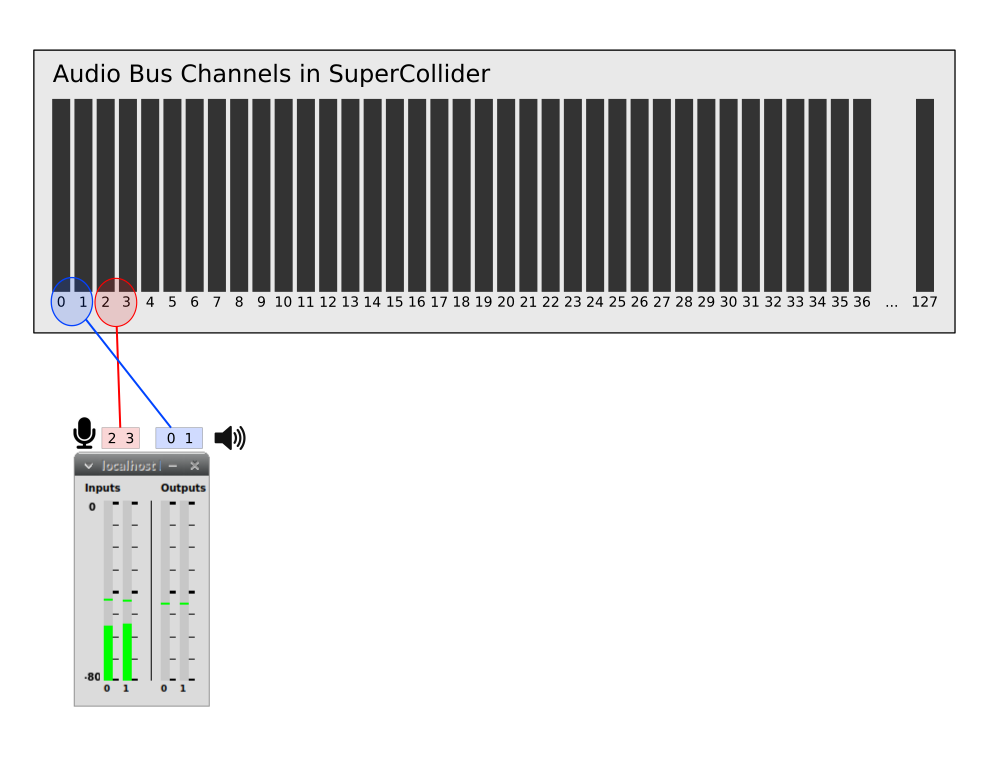
\includegraphics[scale=0.4]{fig-audio-bus-stereo.png}}
\caption{Audio buses and Meter window in SC.}
\label{fig:audio-bus-stereo}
\end{figure}

Hit [ctrl+M] to open up the Meter window. It shows the levels of all inputs and outputs. Figure \ref{fig:audio-bus-stereo} shows a screenshot of this window and its correspondence to SuperCollider's default buses. In SuperCollider, audio buses are numbered from 0 to 127. The first eight (0-7) are by default reserved to be the output channels of your sound card. The next eight (8-15) are reserved for the inputs of your sound card. All the others (16 to 127) are free to be used in any way you want, for example, when you need to route audio signals from one UGen to another.

\subsection{\texttt{Out} and \texttt{In} UGens}

Now try the following line of code:

\begin{lstlisting}[style=SuperCollider-IDE, basicstyle=\scttfamily\footnotesize]
{Out.ar(1, SinOsc.ar(440, 0, 0.1))}.play; // right channel
\end{lstlisting}

The \texttt{Out} UGen takes care of routing signals to specific buses.

The first argument to \texttt{Out} is the target bus, that is, where you want this signal to go.  In the example above, the number \texttt{1} means that we want to send the signal to bus 1, which is the right channel of your sound card.

The second argument of \texttt{Out.ar} is the actual signal that you want to ``write'' into that bus. It can be a single UGen, or a combination of UGens. In the example, it is just a sine wave. You should hear it only on your right speaker (or on your right ear if using headphones).

With the Meter window open and visible, go ahead and change the first argument of \texttt{Out.ar}: try any number between 0 and 7, and watch the meters. You will see that the signal goes wherever you tell it to.

\bigskip
\todo[inline, color=green!40]{ TIP: Most likely you have a sound card that can only play two channels (left and right), so you will only hear the sine tone when you send it to bus 0 or bus 1. When you send it to other buses (3 to 7), you will still see the corresponding meter showing the signal: SC is in fact sending the sound to that bus, but unless you have an 8-channel sound card you will not be able to hear the output of buses 3-7.}
\bigskip

One simple example of an audio bus being used for an effect is shown below.

\begin{lstlisting}[style=SuperCollider-IDE, basicstyle=\scttfamily\footnotesize]
// start the effect
f = {Out.ar(0, BPF.ar(in: In.ar(55), freq: MouseY.kr(1000, 5000), rq: 0.1))}.play;
// start the source
n = {Out.ar(55, WhiteNoise.ar(0.5))}.play;
\end{lstlisting}

The first line declares a synth (stored into the variable \texttt{f}) consisting of a filter UGen (a Band Pass Filter). A band pass filter takes any sound as input, and \emph{filters out all frequencies except the one frequency region that you want to let through}. \texttt{In.ar} is the UGen we use to read from an audio bus; so with \texttt{In.ar(55)} being used as input of the \texttt{BPF}, any sound that we send to bus 55 will be passed to the band pass filter. Notice that this first synth does not make any sound at first: when you evaluate the first line, bus 55 is still empty. It will only make sound when we send some audio into bus 55, which happens on the second line. 

The second line creates a synth and stores it into the variable \texttt{n}. This synth simply generates white noise, and outputs it \emph{not to the loudspeakers directly, but to audio bus 55 instead}. That is precisely the bus that our filter synth is listening to, so as soon as you evaluate the second line, you should start hearing the white noise being filtered by synth \texttt{f}.
In short, the routing looks like this:

\begin{center}
\emph{noise synth} $\rightarrow$ \emph{bus 55} $\rightarrow$ \emph{filter synth}
\end{center}

The order of execution is important. The previous example won't work if you evaluate the source \emph{before} the effect. This will be discussed in more detail in section \ref{sec:order-of-execution}, ``Order of Execution.''

One last thing: when you wrote in earlier examples synths like \texttt{\{SinOsc.ar(440)\}.play}, SC was actually doing \texttt{\{Out.ar(0, SinOsc.ar(440))\}.play} under the hood: it assumed you wanted to send the sound out to bus 0, so it automatically wrapped the first UGen with an \texttt{Out.ar(0, ...)} UGen. In fact a few more things are happening there behind the scenes, but we'll come back to this later (section \ref{sec:synthdef}).
